% !TeX spellcheck = en_US
% !TeX program = xelatex

\documentclass[a4paper,12pt]{article}
\renewcommand{\baselinestretch}{1.2}
\usepackage[utf8]{inputenc}
\usepackage[T2A, T1]{fontenc}
\usepackage[english, russian]{babel}

\usepackage{fontspec}
\setmainfont{Times New Roman}
\usepackage{setspace, amsmath}
\usepackage{amssymb}
\usepackage{dsfont}
\usepackage{epsfig}

\makeatletter
\let\@fnsymbol\@arabic
\makeatother

\usepackage{geometry}
\geometry{
a4paper,
total={170mm, 257mm},
left=20mm,
top=20mm,
}

\usepackage{systeme}
\usepackage{skak}
\usepackage{mathtools}
\usepackage{unicode-math}
\usepackage{array}
\usepackage{makecell}
\usepackage{subfiles}
\usepackage{hyperref}
\hypersetup{pdfstartview=FitH, linkcolor=black, urlcolor=blue, colorlinks=true}
\usepackage{framed}
\usepackage{graphicx}
\usepackage{caption}
\usepackage{subcaption}
\usepackage{color}
\usepackage{chngcntr}
\usepackage{tikz}
\usepackage{csquotes}
\usepackage{fancyhdr}

\pagestyle{fancy}
\fancyhf{}
\fancyhead[L]{\leftmark}
\fancyfoot[C]{\thepage}

\usepackage{float}
\floatstyle{plaintop}
\usepackage{enumitem}
\setlength{\parindent}{0pt}

\graphicspath{{../img/}}
\newcommand{\myPictWidth}{.95\textwidth}
\newcommand{\phm}{\phantom{-}}
\newcommand{\beq}{\begin{equation}}
\newcommand{\eeq}{\end{equation}}


\begin{document}
\tableofcontents
\title{Гидродинамическое моделирование\\Решение задач}
\author{Муравцев А.А. (вариант 16)\thanks{студент группы 5040103/10401; email: almuravcev@yandex.ru}}
\maketitle


\section{Задание 1 от 14.09.2022}
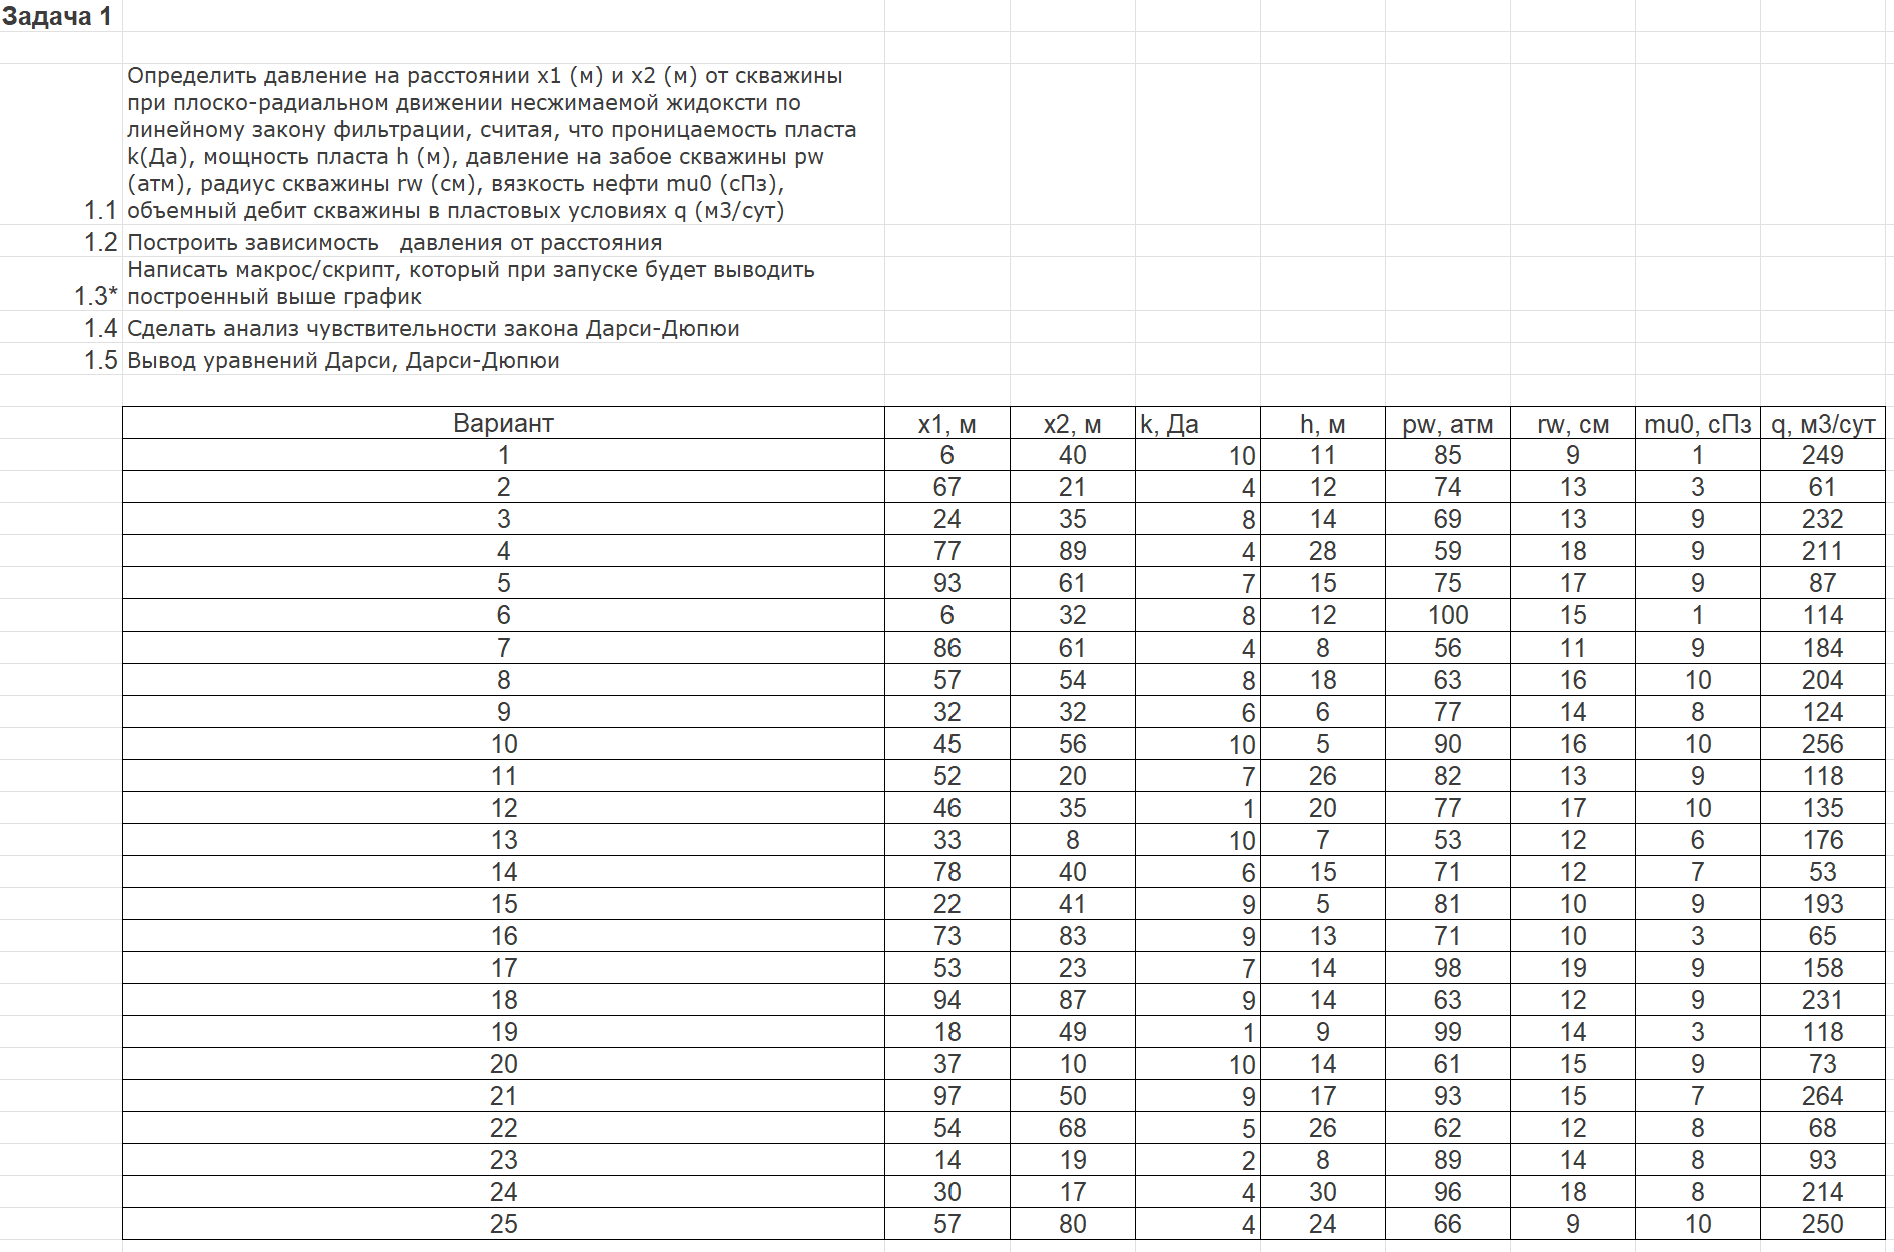
\includegraphics[width=\textwidth]{task1}


\subsection{Расчёт давления по формуле Дюпюи}

Давление на расстоянии $x_1$:
\begin{multline}
P_{x_1}=P_w+\frac{18.41\cdot Q\mu}{kh}\left(\ln{\left(\frac{x_1}{r_w}\right)+S}\right)
=\\=71\text{ атм}+\frac{18.41\cdot 65\dfrac{\text{м}^3}{\text{сут}}\cdot3\text{ сПз}}{9000\text{ мД}\cdot 13\text{ м}}\left(\ln{\left(\frac{73\text{ м}}{0,1\text{ м}}\right)}+0\right)\approx 71.2\text{ атм}
\end{multline}

Давление на расстоянии $x_2$:
\begin{multline}
P_{x_1}=P_w+\frac{18.41\cdot Q\mu}{kh}\left(\ln{\left(\frac{x_2}{r_w}\right)+S}\right)
=\\=71\text{ атм}+\frac{18.41\cdot 65\dfrac{\text{м}^3}{\text{сут}}\cdot3\text{ сПз}}{9000\text{ мД}\cdot 13\text{ м}}\left(\ln{\left(\frac{83\text{ м}}{0,1\text{ м}}\right)}+0\right)\approx 71.2\text{ атм}
\end{multline}


\subsection{График зависимости давления от расстояния}

График зависимости давления от расстояния построен по ссылке: \href{https://colab.research.google.com/github/mualal/notebooks-source/blob/master/6_pressure.ipynb}{Open in Colab}.

\subsection{Макрос для вывода графика}

\subsection{Анализ чувствительности формулы Дюпюи}

\subsection{Вывод уравнения Дарси и формулы Дюпюи}

\section{Задание 2 от 14.09.2022}
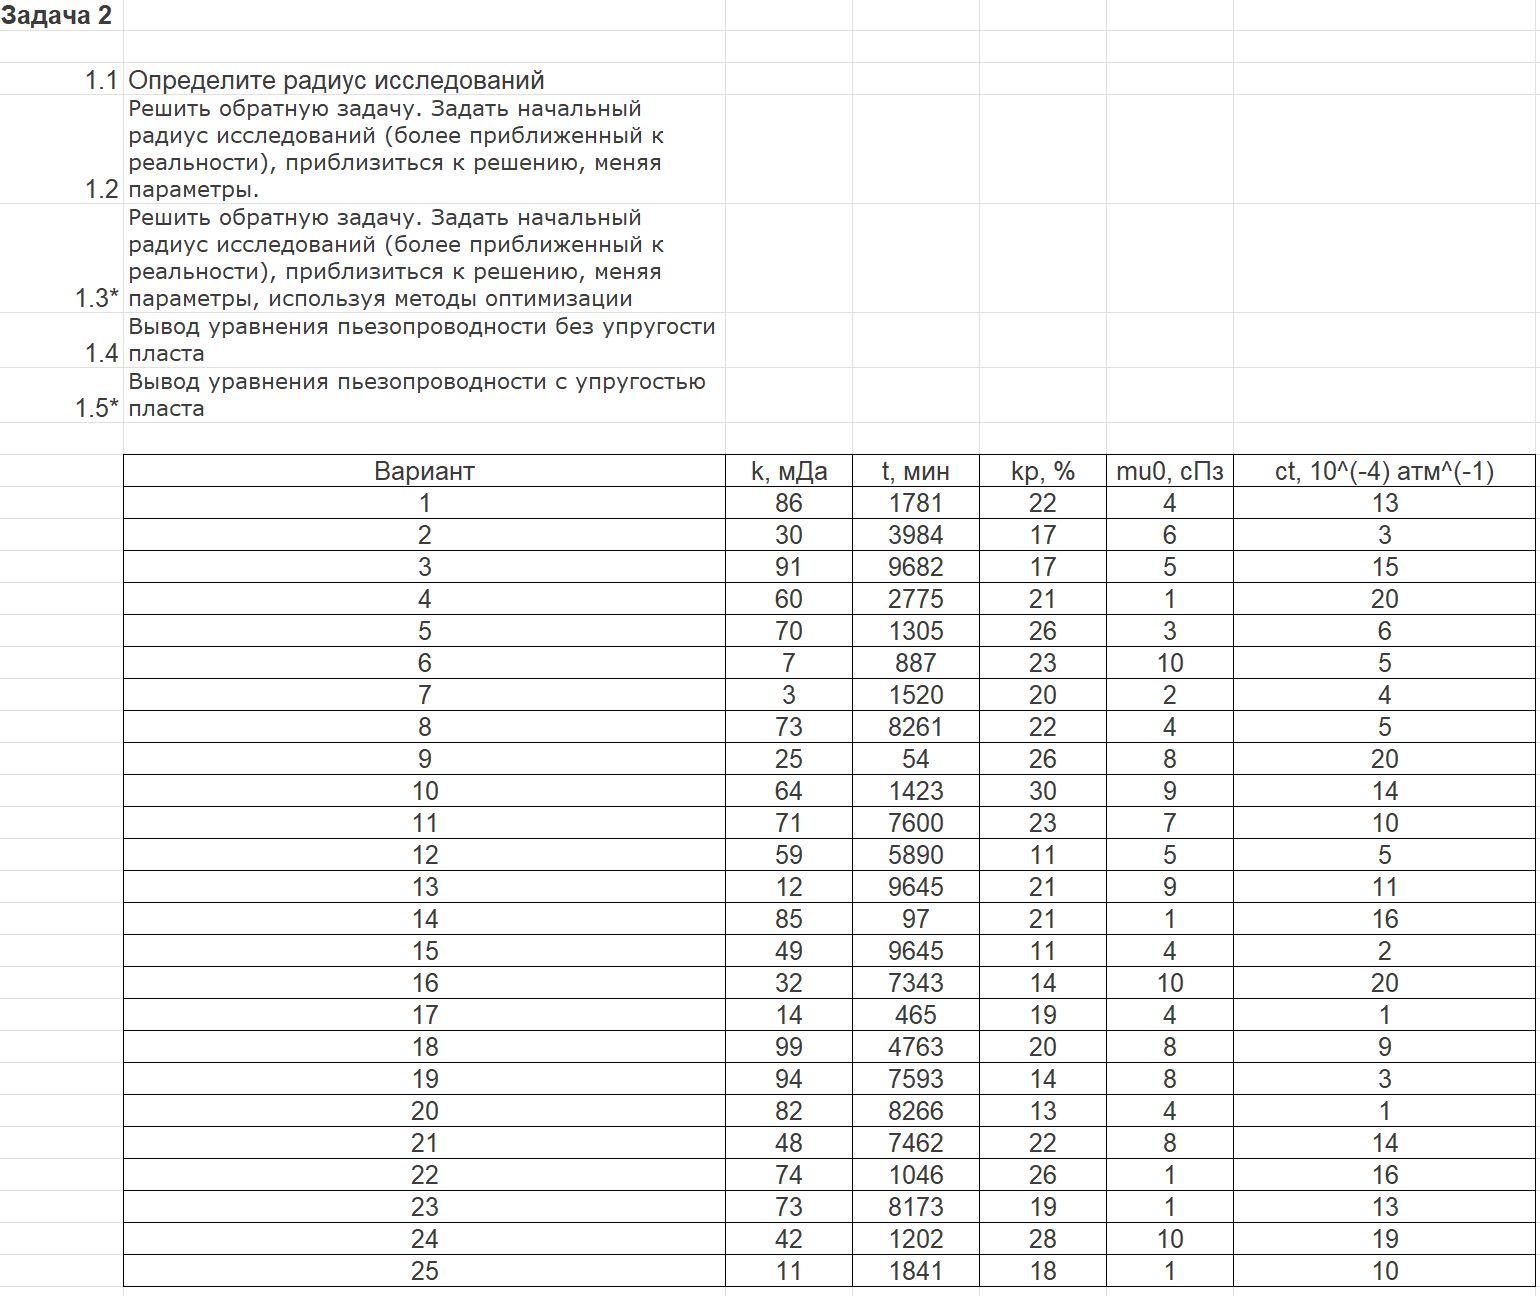
\includegraphics[width=\textwidth]{task2}

\subsection{Радиус исследования}

\subsection{Решение обратной задачи}

\subsection{Вывод уравнения пьезопроводности без упругости пласта}

\subsubsection{В векторной форме (быстрый, но не совсем строгий вывод)}

\subsubsection{В покомпонентной форме с обезразмериванием (от Шеля)}

\subsection{Вывод уравнения пьезопроводности с упругостью пласта}

\section{Задание 1 от 21.09.2022}

\section{Задание 1 от 28.09.2022}

\end{document}
